\documentclass{article}



\usepackage{graphicx}%allows import messages
\usepackage{float}%allow control float position
\usepackage{hyperref}
\hypersetup{ % link to the references e.g. the sections
    colorlinks,
    citecolor=black,
    filecolor=black,
    linkcolor=black,
    urlcolor=black }
%-------------------------------------------------------------------------------------------------------------

\begin{document}
\begin{titlepage}
		\begin{center}% puts the text on the right side of the page
		{\huge{Crownstone protocol V 1.0}}\\ % \\ makes a new line
		[2cm]
		{\large Crownstone B.V }\\
		[15cm]
		\end{center} 
		\begin{flushright}
		{\large Ilhan Delic \\}
		\# 0914619 \\
		november 2019 \\
		\end{flushright}	
\end{titlepage}
% here you can place a summary 
% \section*{Summary}
%text \cleardoublepage 
%-------------------------------------------------------------------------------------------------------------
%table of contents 
\tableofcontents
\thispagestyle{empty}
\cleardoublepage %clears the rest of the page
%-------------------------------------------------------------------------------------------------------------
\pagenumbering{arabic}%the western number system
\section{introduction}\label{sec:intro}% reference
This is the documentation for the protocol for the Crownstone hub. I'll describe my thinking and design process for this protocol. There are a couple of protocol layers in the osi model. When you make an other protocol you add a layer on top of the existing osi model layers. The layers with their corresponding protocols are as follows:\\
\\
1. link layer:  PPP, DSC, Wi-Fi\\
\\
2. internet layer: IPv4, IPv6\\
\\
3. transport layer: TCP, UDP\\
\\
4 application layer: HTTP(/2), IMAP, FTP\\
\\
5 SSE layer: this layer is the methode of data transport that I'll be using for the hub\\
\\
6  My layer: application layer kind of thing. this will be the protocol that I have to make.\\
\\
The protocol should describe the way of communication of the hub with the  cloud and the steps required to this. This document describes the architecture, and functionality the protocol has as well as requirements and tests. The test are documented and describe how it will be tested and what the goal is with the tests. 
\cleardoublepage

%-------------------------------------------------------------------------------------------------------------
\section{Data structure}
The data is send in a JSON file, because the 
The different kinds of data that is being send are: \\
\\
currentLocation:\\
\\
- timestamp: "time now"\\
- user: "string"\\
- user id: "string"\\ 
- current location: \\
\\
\\
currentEnergyUsage:\\
\\
- name of the stone: "string"\\
- energy usage: \\
- duration: \\
- timestamp: "time now"\\
%-------------------------------------------------------------------------------------------------------------
\section{Constraints} 

The server is a entity whose primary responsibilities are: \\
- launch a keep alive stream\\
- get data from the cloud and stream this to the client which requested it\\
- stay connected with the cloud and communicate with it \\
- broker between cloud and client to stream the requested data\\
\\
Client responsibilities  \\
- initiate a connection with the event server\\
- send a request for data\\
\\
Cloud responsibilities  \\
-  the cloud saves the data\\
- provides the data for the server\\ 

%-------------------------------------------------------------------------------------------------------------
\cleardoublepage
\section{Exchange protocol}

\label{fig:protocolDraft}	
	\begin{figure}[H]
	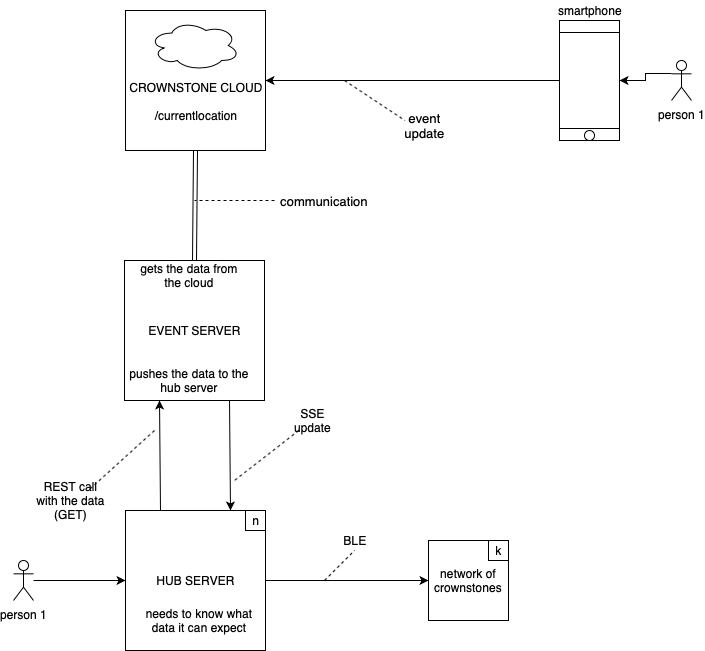
\includegraphics[width=4in]{pictures/prototypeV3.png}
	\caption[Optional caption]{protocol draft design}
	\end{figure}\\
\\
The data exchange all starts at the client when they log in, when logged in you get a token. This token is the identifier of the user, when sending requests to servers the token is being send in as well. This is done so the user won't get someone else's information which is wat we want to prevent. \\
\\
The user can request different kinds of data, like location or energy-usage. Streaming the data is highly useful for data that changes frequently like indoor location or energy-usage. \\
\\
When the token is authenticated which indicates that the users is the correct user and the data stream begins.\\ 
\\
The user can stop the data stream at any time. 
\\
The data is always being updated by your phone which send frequent event updates to the cloud. 
%------------------------------------------------------------------------------------------------------------- 
\section{Authentication}
Authentication is a big part of the protocol. We  can't send the data to the person it is not destined to go too. Therefore the event server needs to function as a filter for returning data. When the server receives a token the sender gets the corresponding data. It is described in this following diagram.\\
	\begin{figure}[H]
	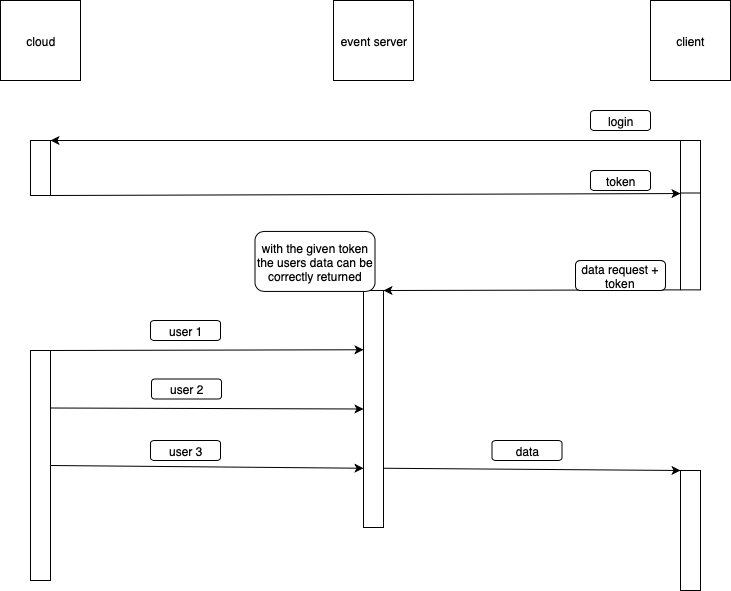
\includegraphics[width=4in]{pictures/authenticationFlow.png}
	\caption[Optional caption]{authentication flow}
	\end{figure}\\

%------------------------------------------------------------------------------------------------------------- 

\section{Architecture}\label{sec:architecture}
The protocol provides a technology for unidirectional data exchange by using SSE. The cloud connects with an Event server. The hub at peoples homes will make a connection(REST call) to the cloud using the evenserver. This architectural style uses SSE and both the server and client can end the connection at a certain point after the start of the connection.  In order to start a connection you need to log in and you account will be authenticated with my \\
\\
%-------------------------------------------------------------------------------------------------------------
\subsection{Structured data}\label{sec:strucdata} \\
SSE require a certain syntax, but on the other hand the cloud has stored data in a certain way as wel. lucky the way the cloud shows its data is with JSON and we can use JSON with SSE. SSE is a keep alive connection until the server or the client leaves the party the data stream won't stop.\\
%-------------------------------------------------------------------------------------------------------------

\subsection{Addresses}\label{sec:addresses} \\
The event server and the client need to be hosted on a certain address that is available. The ES streams the data at that address when the client is connected to that address. when the client is connected it will simply listen to the events until the ether the server or the client breaks the connection. \\
%-------------------------------------------------------------------------------------------------------------

\cleardoublepage
\subsection{Network}\label{sec:network} 
In order to get a better idea of how to set up a protocol i had to make a design of how the communication will flow between the parts. There are three parts: the cloud, the event server and the hub server. \\
\\
The cloud is required to setup the Crownstones: keys and IDs will be generated, and locations can be set. After that, it can be used to add users, so they can also make use of your Crownstones. The cloud is also used to synchronise data between users, and serves as data storage.\\
\\
In order to get the data that's stored on the cloud and show it to the event server, which uses SSE to show the current dynamic data(e.g. current location or the energy usage).\\
 \\
The communication needs to start at the hub side and the hub needs to make a REST call to the cloud in order to start things off. When that has been done the next step would be for the event server to get the data from the cloud. The event server will look at the endpoints with dynamic data like /currentLocation. The event server will put this data in a JSON format and will stream this data to the hub.\\
\\
The data at the cloud is being updated by the smartphones in the Crownstone network. The phone keeps the data at the cloud up to date.  The  data can only be send by the users of the sphere. The sphere is a container of a set of Locations, Stones and Appliances. Every instance of these models has to belong to a sphere so that users can interact with them. Only the users which are members of the sphere owning the Stones can interact with them, be that switching, or just reading the states. These users can send event updates and can view the data from the cloud which is being streamed onto the hub.\\
\\
The hub remains in the sphere just like the other Crownstone objects. It's in the same network with the stones through BLE. \\


\\
%-------------------------------------------------------------------------------------------------------------
\section{functionality} 
 \\
the function of this protocol is to enable the stream of structured data over a network consisting of the Crownstone cloud and several servers. A user needs to log in to the hug. when logged in the user gets a token so the users will be able to get the right data. The data will be picked up from the cloud by the hub, and the hub will stream the data to the connected clients. The data will be streamed using SSE(server send events), with server send events the your data gets automatically updated  every couple of seconds. This is an excellent way to show data that changes often.\\
\\
The hub should be connected with the cloud when the hub is powered on. The hub is in the same sphere as  the other Crownstones, when in the same sphere the hub could easily get the data from the stones. With this way you can only acquire your own data or the data in your sphere.  
\\
the process of getting this data is described like this:\\
Steps on how it wil function \\
\\
Hub  - Cloud: \\
1. The hub is turned on\\
2. The user logs in\\
3. The user gets authenticated\\
4. The hub connects to the cloud\\
5. The connection with the cloud is completed and the hub will show it's connected\\
6. When connected you can enter several commands to get data\\
7. Run the command which runs a bash script to get data stream\\
8. Hub gets the data from the cloud as JSON\\
9. start a SSE stream \\
10. The JSON data will be streamed on the hub and can be picked up by the clients\\
11. When the SSE stream is stoped by client or host there will be a final message to clarify that the connection is dead\\
12. End SSE connection\\

%-------------------------------------------------------------------------------------------------------------
\section{Requirements}\label{sec:requirements}
1: Serialise from/to js/ts\\
Using json to receive data, because we're using ts/js.
the data that is shown in the cloud is also in a json form 
the base JSON streaming layer\\
\\
2: Minimise calls to server(endpoints)\\
make sure the calls to the server are minimised by choosing to stream dynamic data and not static data.\\
\\
3: Dynamic data, data the changes often\\
there is no need for static data, just the dynamic data that changes like location and energy use \\
\\
4: SSE, unidirectional is enough\\
sse is used to stream the dynamic data this is a more efficient way then using websockets\\
\\
5: How many connections simultaneously ? needs to be set
can connect with x clients at a time\\ **************
\\
6: One last message when the communication ends. \\
either form the server or client side but there will be a message if you're not active for a long period of time or when a client ends the connection. \\
\\
7: Making a REST call using the GET methode to get a token and to verify your request with the data you're trying to get is the right data for you.\\
\\
8: The client will be using a token to verify his/her identity when they log in to the cloud\\
\\
9: User is able to choose a certain data stream so you don't get everything at once.\\
\\
10: Able to start/stop data stream at will.\\
\\

%-------------------------------------------------------------------------------------------------------------
\cleardoublepage
\section{Test}\label{sec:test}
This part will describe how the test of the protocol. To make sure the protocol meets the set requirements[\pageref{sec:requirements}].\\
To realise the protocol it should be tested. I don't want to screw up anything with the cloud and i need to start small so I'll host a server on heroku where some dynamic data will be stored. This data will be fetched by a central server and streamed if a client starts a connection. when the client is connected to the central server the data will be streamed until the connection dies at one of the sides. When the stream ends there will be a final message noting that the connection is dead and needs to be reconnected. This is useful is a user isn't active for a long time or if a user chooses to stop the connection him self. This test covers most of the requirements i've set for the protocol. To test if this works with multiple servers i'll make 2 - 3 clients to test this and make it happen. \\
%-------------------------------------------------------------------------------------------------------------

\subsection{Authentication 1}\label{authentication1}
The authentication process for requesting data. When the user is logged in they will get a token for authentication. With this token the user can access the right data(their own).The authentication test uses a program which simulates a register, login and welcome page. \\
\\
step 1.
\\
Start the program called loginclient and open a new tab with the link to localhost:3000.\\
\\
Step 2.
\\
Fill in the fields on the register screen and press enter. You could also press the register button on the page. \\
\\
Step 3. \\
Now you should be registered and you'll be able to log in at the login page. \\
\\
Step 4.\\
Once you've logged in you'll get to the home page. At the homepage you can add or delete(as an owner) other users who can access this data. You can log out at the homepage.\\
\\

The test is a succes if the user is able to log in with the account that was just created
%-------------------------------------------------------------------------------------------------------------
\subsection{Authentication 2}\label{authentication2}

%-------------------------------------------------------------------------------------------------------------

\subsection{One client test}\label{client test}
Step 1. \\
Make sure you've got 3 parts ready the server that functions as a cloud on heroku, the central server that fetches all the data from that heroku server and the client server which starts a connection with the central server to see the data it's streaming. \\
3 parts: \\
heroku server(cloud)\\
non heroku server(central server)\\
non heroku server(hub)\\
\\
Step 2.\\
Activate the heroku server and look at the different endpoints(3 different stones, energy use, energy use history). Change to a different endpoint to see if the data is actually changing. Requirements(which requirements)\\
\\
Step 3.\\
Start the central server to pick up the data that's on the heroku server and stream the data when a client connects. Requirements(which requirements)\\
\\
Step 4. \\
Now start the client. The client wil need to make a REST call first. The REST call is a GET methode so the cloud will know what to expect. It is a automatically search for the central server and connect if it cannot connect the is t will spit out and error but if it does connect it will print connected and start showing data.\\
\\
Step 5. \\
When you are inactive for a long periode of time (1.5 min/ 90 sec.) the connection will close but if you refresh or change an end point the connection should stay alive. there is a possibility for the client to stop the connection as well. \\
\\
The requirements covert in this test are: 
1, 2, 3, 4, 6 and 7.
%-------------------------------------------------------------------------------------------------------------

\subsection{Multiple clients test}\label{mclient}
In the previous test I've covert most requirements there is only 1 left which is the number of maximum connections. SSE with browsers let you use up to 


%-------------------------------------------------------------------------------------------------------------
\cleardoublepage
\section{Research}\label{sec:research} 
To set this document up I was in need of inspiration and needed examples of how other protocols are set up. My supervisor told me to look at the XMPP and the Homie protocols because they are somewhat similar to the protocol i needed to set up. Therefor I took a look at the documents from both protocols to get some inspiration. I also took a look at the Crownstone SDK which 
\\
\subsection{XMPP}\label{sec:xmpp} 
\\
XMPP is the Extensible Messaging and Presence Protocol, a set of open technologies for instant messaging, presence, multi-party chat, voice and video calls, collaboration, lightweight middleware, content syndication, and generalised routing of XML data. This protocol can be a source of inspiration when setting up my own protocol. I will study the documentation so i have an idea on how to set-up mine.\\
\\
At its core, XMPP is a technology for streaming XML over a network. The protocol, which emerged from the Jabber open-source community in 1999, was originally designed to provide an open, secure, decentralised alternative to consumer-oriented instant messaging (IM) services like ICQ, AIM, and MSN. The core technologies were formalised under the name Extensible Messaging and Presence Protocol (XMPP) at the IETF in 2004. These core technologies include:\\
\\
- The base XML streaming layer\\
- Channel encryption using Transport Layer Security (TLS)\\
- Strong authentication using the Simple Authentication and Security Layer (SASL)\\
- Use of UTF-8 for complete Unicode support, including fully internationalised addresses\\
- Built-in information about network availability (“presence”)\\
- Presence subscriptions for two-way authorization\\
- Presence-enabled contact lists (“rosters”)\\
\\
The format used in the XMPP documentation was really useful to get a sense of what to make of the protocol documentation. It helped setting up a couple of chapters. 

\cleardoublepage
\subsection{MQTT Homie}\label{sec:homie}
\\
MQTT supports easy and unrestricted message-based communication.\\
\\
However, MQTT doesn't define the structure and content of these messages and their relation. An IoT device publishes data and provides interaction possibilities but a controlling entity will need to be specifically configured to be able to interface with the device.\\
\\
The Homie convention defines a standardized way of how IoT devices and services announce themselves and their data on the MQTT broker.\\
\\
It is thereby a crucial aspect on top of the MQTT protocol for automatic discovery, configuration and usage of devices and services.
\\
\subsection{Crownstone SDK}\label{sec:CSDK}\\
\\
The Crownstone rest api is running on heroku and is available at https://cloud.crownstone.rocks. The base url for the rest api is https://cloud.crownstone.rocks/api. The endpoints are then appended to the base url. E.g. POST /users/login becomes POST https://cloud.crownstone.rocks/api/users/login. Note, navigating to that URL won't work. It's a POST request. If you want to use the POST login command, make sure you do not use an access token in this request.\\
\\
To explore the API login through: https://cloud.crownstone.rocks/ and copy the accessToken to the explorer. The explorer gives an overview of the available endpoints and can be found at https://cloud.crownstone.rocks/explorer/. The endpoints describe the parameters as well as the responses.\\
\\
To get a better view of how to get data from the cloud I used the Crownstone SDK. With this I could see the endpoints which were required for the different data. Such as current location, energy use history and current energy use. Knowing which endpoints to use  is essential in getting to the correct data.\\ 

%-------------------------------------------------------------------------------------------------------------
\cleardoublepage
\section{References}\label{sec:references}

XMPP:\\
Extensible Messaging and Presence Protocol (XMPP): Core\\
P. Saint-Andre\\
ISSN: 2070-1721\\
March 2011\\
https://xmpp.org/rfcs/rfc6120.html \\
\\
Crownstone SDK: \\
https://github.com/crownstone/crownstone-sdk\\
https://github.com/crownstone/crownstone-sdk/blob/master/REST_API.md\\
September 2019\\
\\
MQTT Homie:\\
https://homieiot.github.io/\\
July 2019\\
V4.0\\
\\
SSE:\\
https://www.w3.org/TR/2009/WD-eventsource-20090421/\\

%-------------------------------------------------------------------------------------------------------------
\end{document}